\pdfbookmark[0]{Figure 1}{comparison:1}
{\Large\bfseries Figure 1: Seismicity and ground displacement}\par\medskip
\begin{minipage}[t]{.485\textwidth}\vspace{0pt}\centering
{\large\bfseries Published reference}\par\medskip
\includegraphics[width=\linewidth,height=5.85in,keepaspectratio]{report/reference_assets/F1.png}
\par\smallskip{\footnotesize Tan et al. (2025), tanmodel.pdf, p. 2.\par DOI: 10.1126/science.adw9038.}
\end{minipage}\hfill
\begin{minipage}[t]{.485\textwidth}\vspace{0pt}\centering
{\large\bfseries Independent result}\par\medskip
\textbf{Panel 1B --- partially reproduced}\par\smallskip
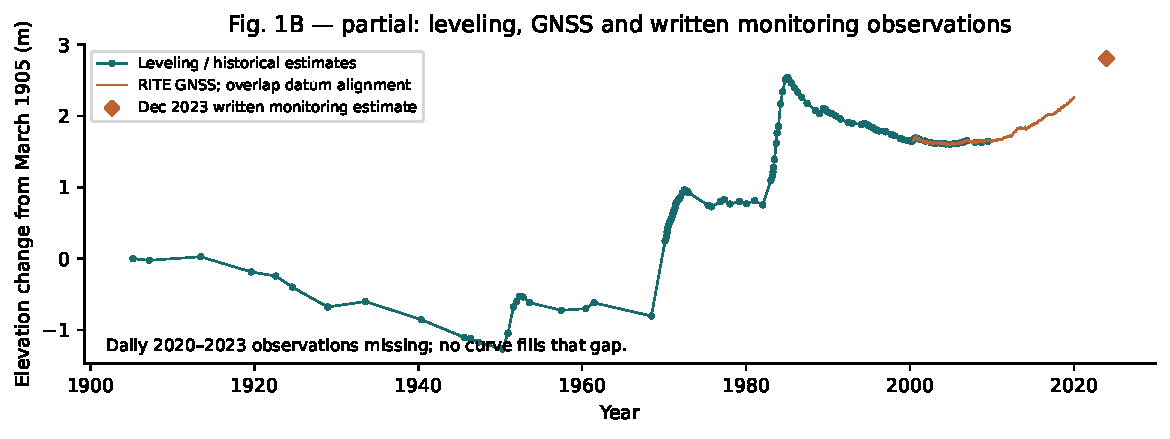
\includegraphics[width=\linewidth,height=4.3in,keepaspectratio]{figures/historical_leveling_partial.pdf}
\par\smallskip{\small Panel 1B is partial: original leveling through 2009 and daily GNSS through 2019, with a separate written December 2023 monitoring endpoint. The vertical datum is relative to March 1905; daily observations for 2020--2023 are missing.}\par\medskip
\unavailable{Panels A and C}{Panels 1A and 1C have no valid independent counterpart; existing routine-catalog plots are external context.}
\end{minipage}
\vfill
\newpage
\pdfbookmark[0]{Figure 2}{comparison:2}
{\Large\bfseries Figure 2: Temporal evolution of seismicity}\par\medskip
\begin{minipage}[t]{.485\textwidth}\vspace{0pt}\centering
{\large\bfseries Published reference}\par\medskip
\includegraphics[width=\linewidth,height=5.85in,keepaspectratio]{report/reference_assets/F2.png}
\par\smallskip{\footnotesize Tan et al. (2025), tanmodel.pdf, p. 3.\par DOI: 10.1126/science.adw9038.}
\end{minipage}\hfill
\begin{minipage}[t]{.485\textwidth}\vspace{0pt}\centering
{\large\bfseries Independent result}\par\medskip
\unavailable{All panels/views}{Panels A and B require a multiyear calibrated, relocated catalog and magnitudes. Only nine provisional associations exist.}
\end{minipage}
\vfill
\newpage
\pdfbookmark[0]{Figure 3}{comparison:3}
{\Large\bfseries Figure 3: Spatial distribution of seismicity}\par\medskip
\begin{minipage}[t]{.485\textwidth}\vspace{0pt}\centering
{\large\bfseries Published reference}\par\medskip
\includegraphics[width=\linewidth,height=5.85in,keepaspectratio]{report/reference_assets/F3.png}
\par\smallskip{\footnotesize Tan et al. (2025), tanmodel.pdf, p. 4.\par DOI: 10.1126/science.adw9038.}
\end{minipage}\hfill
\begin{minipage}[t]{.485\textwidth}\vspace{0pt}\centering
{\large\bfseries Independent result}\par\medskip
\unavailable{All panels/views}{The map and both cross sections require independently calibrated and double-difference-relocated events. Provisional diagnostic locations are not substitutes.}
\end{minipage}
\vfill
\newpage
\pdfbookmark[0]{Figure 4}{comparison:4}
{\Large\bfseries Figure 4: Focal mechanisms of larger events}\par\medskip
\begin{minipage}[t]{.485\textwidth}\vspace{0pt}\centering
{\large\bfseries Published reference}\par\medskip
\includegraphics[width=\linewidth,height=5.85in,keepaspectratio]{report/reference_assets/F4.png}
\par\smallskip{\footnotesize Tan et al. (2025), tanmodel.pdf, p. 5.\par DOI: 10.1126/science.adw9038.}
\end{minipage}\hfill
\begin{minipage}[t]{.485\textwidth}\vspace{0pt}\centering
{\large\bfseries Independent result}\par\medskip
\unavailable{All panels/views}{Panels A and B require independent SKHASH/gCAP solutions and reliable locations. No focal inversion was executed.}
\end{minipage}
\vfill
\newpage
\pdfbookmark[0]{Figure S1}{comparison:S1}
{\Large\bfseries Figure S1: Recorded station availability}\par\medskip
\begin{minipage}[t]{.485\textwidth}\vspace{0pt}\centering
{\large\bfseries Published reference}\par\medskip
\includegraphics[width=\linewidth,height=5.85in,keepaspectratio]{report/reference_assets/FS1.png}
\par\smallskip{\footnotesize Tan et al. (2025), tanmodelsupp.pdf, p. 12.\par DOI: 10.1126/science.adw9038.}
\end{minipage}\hfill
\begin{minipage}[t]{.485\textwidth}\vspace{0pt}\centering
{\large\bfseries Independent result}\par\medskip
\textbf{Panel S1 --- partially reproduced}\par\smallskip
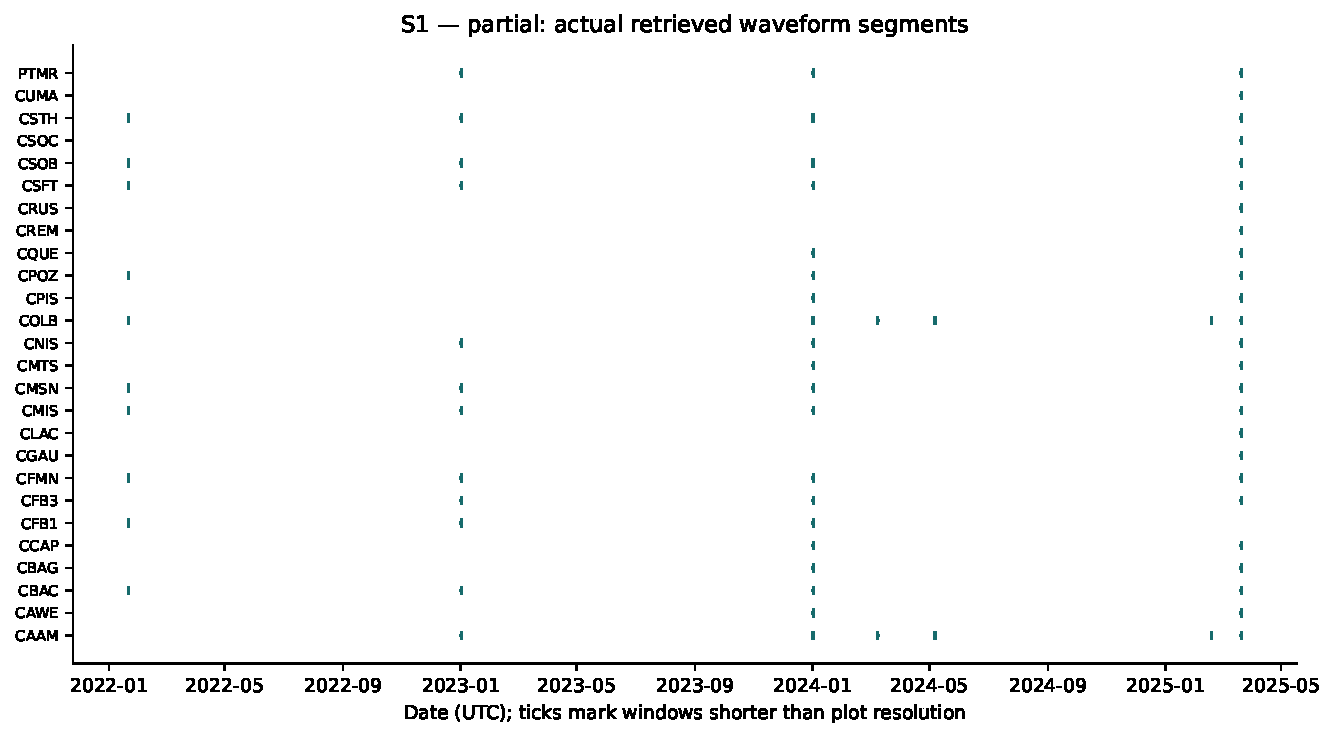
\includegraphics[width=\linewidth,height=4.3in,keepaspectratio]{figures/coverage_partial.pdf}
\par\smallskip{\small Partial: actual returned waveform intervals from 171 files and 26 station names. Short retrieved windows are marked without implying continuous coverage between them; channel-hours are not full network-years.}\par\medskip
\end{minipage}
\vfill
\newpage
\pdfbookmark[0]{Figure S2}{comparison:S2}
{\Large\bfseries Figure S2: Station locations}\par\medskip
\begin{minipage}[t]{.485\textwidth}\vspace{0pt}\centering
{\large\bfseries Published reference}\par\medskip
\includegraphics[width=\linewidth,height=5.85in,keepaspectratio]{report/reference_assets/FS2.png}
\par\smallskip{\footnotesize Tan et al. (2025), tanmodelsupp.pdf, p. 13.\par DOI: 10.1126/science.adw9038.}
\end{minipage}\hfill
\begin{minipage}[t]{.485\textwidth}\vspace{0pt}\centering
{\large\bfseries Independent result}\par\medskip
\textbf{Panel S2 --- partially reproduced}\par\smallskip
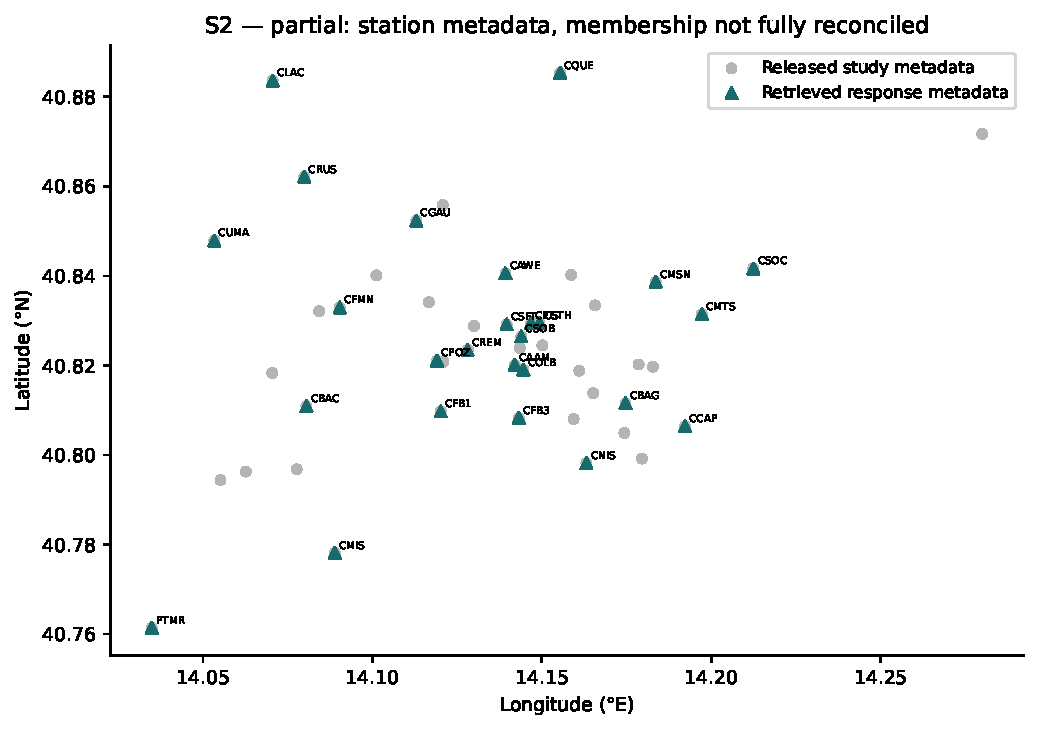
\includegraphics[width=\linewidth,height=4.3in,keepaspectratio]{figures/stations_partial.pdf}
\par\smallskip{\small Partial: released station coordinates and retrieved IV/2I response metadata. Exact membership of the original 48 instruments, station epochs and the basemap are not fully reconciled.}\par\medskip
\end{minipage}
\vfill
\newpage
\pdfbookmark[0]{Figure S3}{comparison:S3}
{\Large\bfseries Figure S3: Training examples}\par\medskip
\begin{minipage}[t]{.485\textwidth}\vspace{0pt}\centering
{\large\bfseries Published reference}\par\medskip
\includegraphics[width=\linewidth,height=5.85in,keepaspectratio]{report/reference_assets/FS3.png}
\par\smallskip{\footnotesize Tan et al. (2025), tanmodelsupp.pdf, p. 14.\par DOI: 10.1126/science.adw9038.}
\end{minipage}\hfill
\begin{minipage}[t]{.485\textwidth}\vspace{0pt}\centering
{\large\bfseries Independent result}\par\medskip
\unavailable{All panels/views}{Panels A--D require the specified training traces, annotations and augmentation examples. These were not reconstructed; downstream use of trained weights is not retraining.}
\end{minipage}
\vfill
\newpage
\pdfbookmark[0]{Figure S4}{comparison:S4}
{\Large\bfseries Figure S4: PhaseNet benchmark examples}\par\medskip
\begin{minipage}[t]{.485\textwidth}\vspace{0pt}\centering
{\large\bfseries Published reference}\par\medskip
\includegraphics[width=\linewidth,height=5.85in,keepaspectratio]{report/reference_assets/FS4.png}
\par\smallskip{\footnotesize Tan et al. (2025), tanmodelsupp.pdf, p. 15.\par DOI: 10.1126/science.adw9038.}
\end{minipage}\hfill
\begin{minipage}[t]{.485\textwidth}\vspace{0pt}\centering
{\large\bfseries Independent result}\par\medskip
\unavailable{All panels/views}{Panels A and B were not generated for the exact CSOB swarm and CMIS noise examples. Other unlabeled inference comparisons remain diagnostics.}
\end{minipage}
\vfill
\newpage
\pdfbookmark[0]{Figure S5}{comparison:S5}
{\Large\bfseries Figure S5: Routine-catalog locations}\par\medskip
\begin{minipage}[t]{.485\textwidth}\vspace{0pt}\centering
{\large\bfseries Published reference}\par\medskip
\includegraphics[width=\linewidth,height=5.85in,keepaspectratio]{report/reference_assets/FS5.png}
\par\smallskip{\footnotesize Tan et al. (2025), tanmodelsupp.pdf, p. 16.\par DOI: 10.1126/science.adw9038.}
\end{minipage}\hfill
\begin{minipage}[t]{.485\textwidth}\vspace{0pt}\centering
{\large\bfseries Independent result}\par\medskip
\unavailable{All panels/views}{Current INGV routine-catalog plots are external context. The saved panel record contains no valid independent counterpart to these three views; the published selection/version is unresolved.}
\end{minipage}
\vfill
\newpage
\pdfbookmark[0]{Figure S6}{comparison:S6}
{\Large\bfseries Figure S6: Initial VELEST locations}\par\medskip
\begin{minipage}[t]{.485\textwidth}\vspace{0pt}\centering
{\large\bfseries Published reference}\par\medskip
\includegraphics[width=\linewidth,height=5.85in,keepaspectratio]{report/reference_assets/FS6.png}
\par\smallskip{\footnotesize Tan et al. (2025), tanmodelsupp.pdf, p. 17.\par DOI: 10.1126/science.adw9038.}
\end{minipage}\hfill
\begin{minipage}[t]{.485\textwidth}\vspace{0pt}\centering
{\large\bfseries Independent result}\par\medskip
\unavailable{All panels/views}{The map and both cross sections require scientific VELEST location and velocity/station-correction runs. Compilation alone did not produce these results.}
\end{minipage}
\vfill
\newpage
\pdfbookmark[0]{Figure S7}{comparison:S7}
{\Large\bfseries Figure S7: Location uncertainties}\par\medskip
\begin{minipage}[t]{.485\textwidth}\vspace{0pt}\centering
{\large\bfseries Published reference}\par\medskip
\includegraphics[width=\linewidth,height=5.85in,keepaspectratio]{report/reference_assets/FS7.png}
\par\smallskip{\footnotesize Tan et al. (2025), tanmodelsupp.pdf, p. 18.\par DOI: 10.1126/science.adw9038.}
\end{minipage}\hfill
\begin{minipage}[t]{.485\textwidth}\vspace{0pt}\centering
{\large\bfseries Independent result}\par\medskip
\unavailable{All panels/views}{Panels A--G require independently selected regional subsets, HypoDD SVD locations and coordinate uncertainties. None of these scientific inversions ran.}
\end{minipage}
\vfill
\newpage
\pdfbookmark[0]{Figure S8}{comparison:S8}
{\Large\bfseries Figure S8: Magnitude calibration and frequency distribution}\par\medskip
\begin{minipage}[t]{.485\textwidth}\vspace{0pt}\centering
{\large\bfseries Published reference}\par\medskip
\includegraphics[width=\linewidth,height=5.85in,keepaspectratio]{report/reference_assets/FS8.png}
\par\smallskip{\footnotesize Tan et al. (2025), tanmodelsupp.pdf, p. 19.\par DOI: 10.1126/science.adw9038.}
\end{minipage}\hfill
\begin{minipage}[t]{.485\textwidth}\vspace{0pt}\centering
{\large\bfseries Independent result}\par\medskip
\unavailable{All panels/views}{Panels A and B require qualifying relative-amplitude equations and calibrated magnitudes. Zero qualifying equations were obtained; completeness and b-value were not estimated.}
\end{minipage}
\vfill
\newpage
\pdfbookmark[0]{Figure S9}{comparison:S9}
{\Large\bfseries Figure S9: Best-located earthquake subset}\par\medskip
\begin{minipage}[t]{.485\textwidth}\vspace{0pt}\centering
{\large\bfseries Published reference}\par\medskip
\includegraphics[width=\linewidth,height=5.85in,keepaspectratio]{report/reference_assets/FS9.png}
\par\smallskip{\footnotesize Tan et al. (2025), tanmodelsupp.pdf, p. 20.\par DOI: 10.1126/science.adw9038.}
\end{minipage}\hfill
\begin{minipage}[t]{.485\textwidth}\vspace{0pt}\centering
{\large\bfseries Independent result}\par\medskip
\unavailable{All panels/views}{All three views require independently relocated events and cross-correlation observation counts for the published quality filter. These outputs are absent.}
\end{minipage}
\vfill
\newpage
\pdfbookmark[0]{Figure S10}{comparison:S10}
{\Large\bfseries Figure S10: Seismicity by year}\par\medskip
\begin{minipage}[t]{.485\textwidth}\vspace{0pt}\centering
{\large\bfseries Published reference}\par\medskip
\includegraphics[width=\linewidth,height=5.85in,keepaspectratio]{report/reference_assets/FS10.png}
\par\smallskip{\footnotesize Tan et al. (2025), tanmodelsupp.pdf, p. 21.\par DOI: 10.1126/science.adw9038.}
\end{minipage}\hfill
\begin{minipage}[t]{.485\textwidth}\vspace{0pt}\centering
{\large\bfseries Independent result}\par\medskip
\unavailable{All panels/views}{The four annual groups for 2022--2025 require the independent multiyear relocated catalog. The available sample does not support them.}
\end{minipage}
\vfill
\newpage
\pdfbookmark[0]{Figure S11}{comparison:S11}
{\Large\bfseries Figure S11: Four major swarms}\par\medskip
\begin{minipage}[t]{.485\textwidth}\vspace{0pt}\centering
{\large\bfseries Published reference}\par\medskip
\includegraphics[width=\linewidth,height=5.85in,keepaspectratio]{report/reference_assets/FS11.png}
\par\smallskip{\footnotesize Tan et al. (2025), tanmodelsupp.pdf, p. 22.\par DOI: 10.1126/science.adw9038.}
\end{minipage}\hfill
\begin{minipage}[t]{.485\textwidth}\vspace{0pt}\centering
{\large\bfseries Independent result}\par\medskip
\unavailable{All panels/views}{The four swarm maps require the independent relocated catalog and justified swarm windows. These selections and locations remain incomplete.}
\end{minipage}
\vfill
\newpage
\pdfbookmark[0]{Figure S12}{comparison:S12}
{\Large\bfseries Figure S12: Ring sectors and CPOZ common-receiver gathers}\par\medskip
\begin{minipage}[t]{.485\textwidth}\vspace{0pt}\centering
{\large\bfseries Published reference}\par\medskip
\includegraphics[width=\linewidth,height=5.85in,keepaspectratio]{report/reference_assets/FS12.png}
\par\smallskip{\footnotesize Tan et al. (2025), tanmodelsupp.pdf, p. 23.\par DOI: 10.1126/science.adw9038.}
\end{minipage}\hfill
\begin{minipage}[t]{.485\textwidth}\vspace{0pt}\centering
{\large\bfseries Independent result}\par\medskip
\unavailable{All panels/views}{Panels A--H require relocated sector selections and independently associated CPOZ P arrivals. The current associations contain zero CPOZ P arrivals.}
\end{minipage}
\vfill
\newpage
\pdfbookmark[0]{Figure S13}{comparison:S13}
{\Large\bfseries Figure S13: Relocated seismicity on satellite imagery}\par\medskip
\begin{minipage}[t]{.485\textwidth}\vspace{0pt}\centering
{\large\bfseries Published reference}\par\medskip
\includegraphics[width=\linewidth,height=5.85in,keepaspectratio]{report/reference_assets/FS13.png}
\par\smallskip{\footnotesize Tan et al. (2025), tanmodelsupp.pdf, p. 24.\par DOI: 10.1126/science.adw9038.}
\end{minipage}\hfill
\begin{minipage}[t]{.485\textwidth}\vspace{0pt}\centering
{\large\bfseries Independent result}\par\medskip
\unavailable{All panels/views}{Panels A and B require reliable independent relocated coordinates and an appropriately sourced basemap. The relocated catalog does not exist.}
\end{minipage}
\vfill
\newpage
\pdfbookmark[0]{Figure S14}{comparison:S14}
{\Large\bfseries Figure S14: Hybrid-event clusters}\par\medskip
\begin{minipage}[t]{.485\textwidth}\vspace{0pt}\centering
{\large\bfseries Published reference}\par\medskip
\includegraphics[width=\linewidth,height=5.85in,keepaspectratio]{report/reference_assets/FS14.png}
\par\smallskip{\footnotesize Tan et al. (2025), tanmodelsupp.pdf, p. 25.\par DOI: 10.1126/science.adw9038.}
\end{minipage}\hfill
\begin{minipage}[t]{.485\textwidth}\vspace{0pt}\centering
{\large\bfseries Independent result}\par\medskip
\unavailable{All panels/views}{The three clusters and unclustered group require a multiyear scan, confirmed events, frequency indices and cluster-relative magnitudes. Four current candidates are unconfirmed.}
\end{minipage}
\vfill
\newpage
\pdfbookmark[0]{Figure S15}{comparison:S15}
{\Large\bfseries Figure S15: Hybrid and shallow-event waveforms}\par\medskip
\begin{minipage}[t]{.485\textwidth}\vspace{0pt}\centering
{\large\bfseries Published reference}\par\medskip
\includegraphics[width=\linewidth,height=5.85in,keepaspectratio]{report/reference_assets/FS15.png}
\par\smallskip{\footnotesize Tan et al. (2025), tanmodelsupp.pdf, p. 26.\par DOI: 10.1126/science.adw9038.}
\end{minipage}\hfill
\begin{minipage}[t]{.485\textwidth}\vspace{0pt}\centering
{\large\bfseries Independent result}\par\medskip
\textbf{Panel S15C --- partially reproduced}\par\smallskip
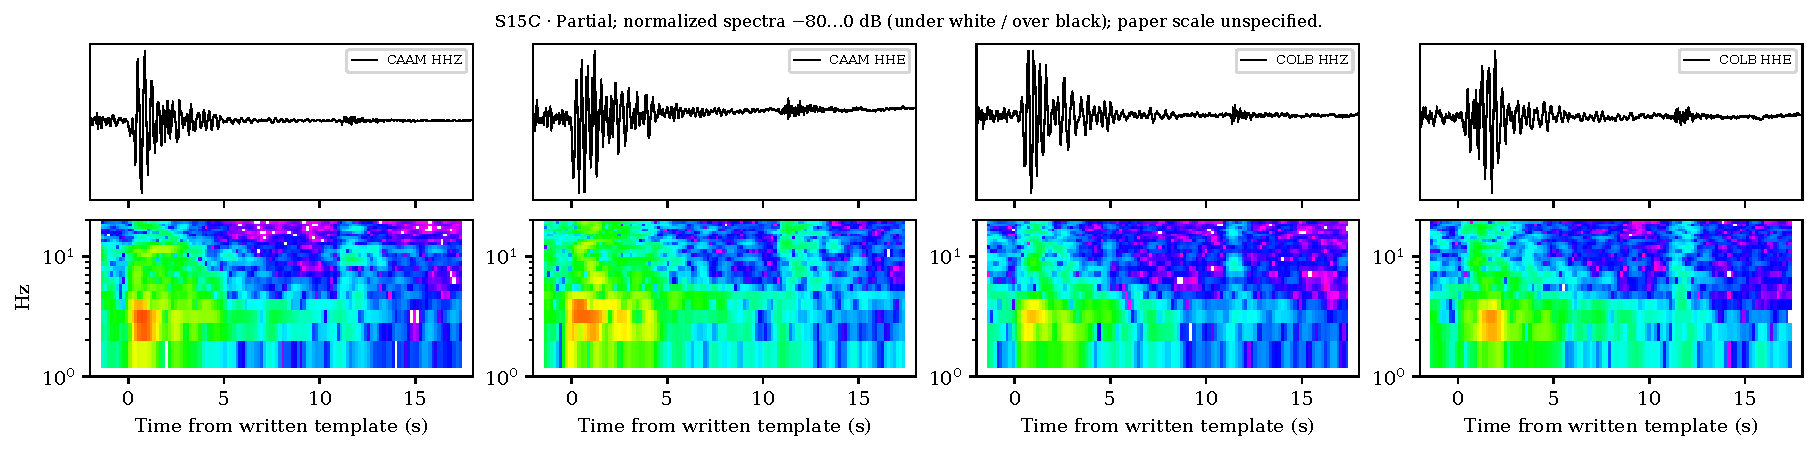
\includegraphics[width=\linewidth,height=4.3in,keepaspectratio]{figures/hybrid_E3.pdf}
\par\smallskip{\small Panel C is partial: independently processed E3 CAAM/COLB observations. Onset alignment, display filtering and spectral settings differ or are incompletely specified. A, B and D have placeholders rather than substitute waveforms.}\par\medskip
\unavailable{Panels A, B and D}{Panels A and B use different published events from the saved E1/E2 templates; D has no independently selected matching example. Those panels remain not reproduced.}
\end{minipage}
\vfill
\newpage
